\begin{figure*}
	\centering
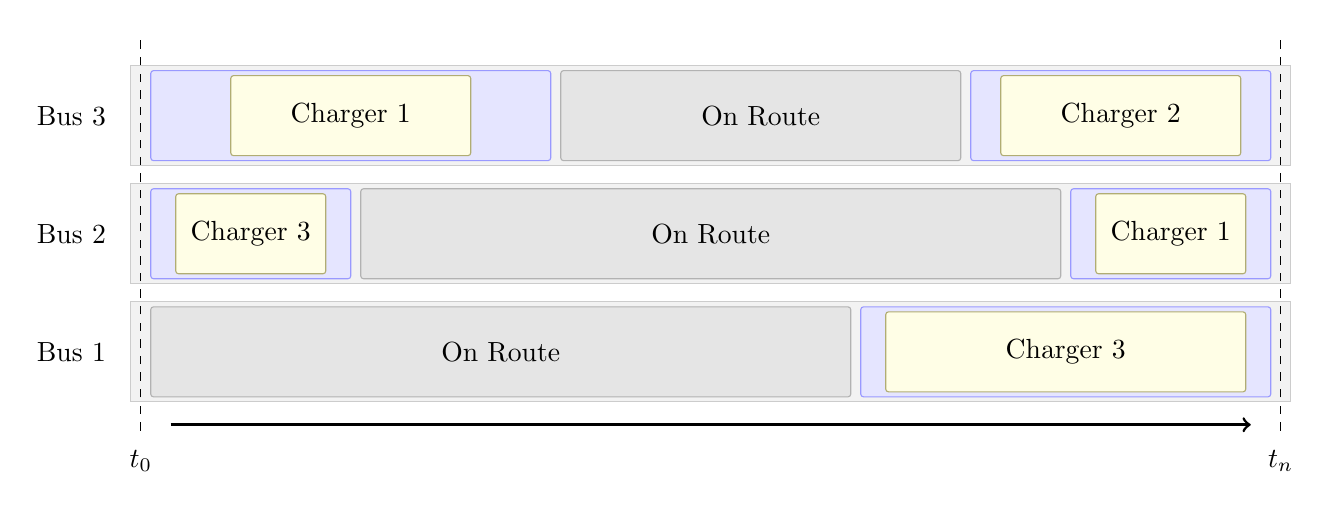
\begin{tikzpicture}
	\node[rectangle, draw=gray!40, fill=gray!10, minimum width=5.8in, minimum height=0.5in](charger1Box) at (3in,1){};
	\node(bus1BoxLabel) at (-0.5, 1){Bus 1}; 

	\node[rectangle, draw=gray!40, fill=gray!10, minimum width=5.8in, minimum height=0.5in](charger2Box) at (3in,2.5){};
	\node(bus1BoxLabel) at (-0.5, 2.5){Bus 2};

	\node[rectangle, draw=gray!40, fill=gray!10, minimum width=5.8in, minimum height=0.5in](charger3Box) at (3in,4){};
	\node(bus1BoxLabel) at (-0.5, 4){Bus 3};

	\node[label=below:$t_0$](origin) at (0.15in,0){};
	\node(xAxes) at (0.15in,5){};
	\node[label=below:$t_n$](bottomRight) at (5.85in,0){};
	\node(topRight) at (5.85in,5){};
	\draw[dashed, line width=0.5pt] (origin.center) -- (xAxes.center); 
	\draw[dashed, line width=0.5pt] (bottomRight.center) -- (topRight.center);
	\node(t0) at (0.3in,-0.05){};
	\node(tn) at (5.7in,-0.05){};
	\draw[->, line width=1pt] (t0.north) -- (tn.north); 

	% draw bus 3 boxes
	\node[rectangle, draw=blue!40, fill=blue!10, minimum width=2in, minimum height=0.45in, rounded corners=1pt](bus1Avail1) at (1.2in,4){};
	\node[rectangle, draw=yellow!50!black!70, fill=yellow!10, minimum width=1.2in, minimum height=0.4in, rounded corners=1pt](bus1Time1) at (1.2in,4){Charger 1};

	\node[rectangle, draw=black!30, fill=black!10, minimum width=2in, minimum height=0.45in, rounded corners=1pt](bus2Time1) at (3.25in,4){On Route};

	\node[rectangle, draw=blue!40, fill=blue!10, minimum width=1.5in, minimum height=0.45in, rounded corners=1pt](bus1Avail1) at (5.05in,4){};
	\node[rectangle, draw=yellow!50!black!70, fill=yellow!10, minimum width=1.2in, minimum height=0.40in, rounded corners=1pt](bus3Time1) at (5.05in,4){Charger 2};

	% draw bus 2 boxes
	\node[rectangle, draw=blue!40, fill=blue!10, minimum width=1in, minimum height=0.45in, rounded corners=1pt](bus1Avail1) at (0.7in,2.5){};
	\node[rectangle, draw=yellow!50!black!70, fill=yellow!10, minimum width=0.75in, minimum height=0.4in, rounded corners=1pt](free1) at (0.7in,2.5){Charger 3};

	\node[rectangle, draw=black!30, fill=black!10, minimum width=3.5in, minimum height=0.45in, rounded corners=1pt](bus3Time2) at (3.0in,2.5){On Route};

	\node[rectangle, draw=blue!40, fill=blue!10, minimum width=1.0in, minimum height=0.45in, rounded corners=1pt](bus1Avail1) at (5.3in,2.5){};
	\node[rectangle, draw=yellow!50!black!70, fill=yellow!10, minimum width=0.75in, minimum height=0.4in, rounded corners=1pt](free2) at (5.3in,2.5){Charger 1};

	% draw bus 1 boxes 
	\node[rectangle, draw=black!30!, fill=black!10, minimum width=3.5in, minimum height=0.45in, rounded corners=1pt](bus3Time2) at (1.95in,1){On Route}; 

	\node[rectangle, draw=blue!40, fill=blue!10, minimum width=2.05in, minimum height=0.45in, rounded corners=1pt](bus1Avail1) at (4.775in,1){};
	\node[rectangle, draw=yellow!50!black!70, fill=yellow!10, minimum width=1.8in, minimum height=0.4in, rounded corners=1pt](bus1Time2) at (4.775in,1){Charger 3};
\end{tikzpicture}
	\caption{Reserving time slots on chargers}
	\label{fig:busTime4}
\end{figure*}
